\documentclass[11pt]{article}
% Shared preamble for report.tex and summary.tex (pdflatex, single column, US letter).
\usepackage[T1]{fontenc}
\usepackage[utf8]{inputenc}
\usepackage{lmodern}
\usepackage[letterpaper, margin=1in]{geometry}
\usepackage[final]{microtype}
\usepackage{amsmath, amssymb}
\usepackage{textcomp}
\usepackage{newunicodechar}
\newunicodechar{η}{\ensuremath{\eta}}
\newunicodechar{±}{\ensuremath{\pm}}
\newunicodechar{×}{\ensuremath{\times}}
\newunicodechar{→}{\ensuremath{\rightarrow}}
\newunicodechar{·}{\textperiodcentered}
\newunicodechar{⁷}{\textsuperscript{7}}
\newunicodechar{⁸}{\textsuperscript{8}}
\usepackage{graphicx}
\usepackage{xcolor}
\definecolor{fkgblue}{HTML}{2F6FBF}
\usepackage{booktabs, array, tabularx, xltabular, makecell}
\renewcommand{\arraystretch}{1.18}
\setlength{\tabcolsep}{5pt}
\usepackage{enumitem}
\setlist{itemsep=2pt, topsep=4pt, leftmargin=1.4em}
\usepackage[font=small, labelfont=bf, margin=0pt]{caption}
\usepackage{float}
\usepackage{tikz}
\usetikzlibrary{arrows.meta, positioning, fit, backgrounds, calc}
\usepackage{listings}
\lstdefinestyle{base}{basicstyle=\ttfamily\footnotesize, columns=fullflexible, keepspaces=true, breaklines=true,
  breakatwhitespace=false, frame=single, rulecolor=\color{black!25},
  framesep=4pt, xleftmargin=4pt, xrightmargin=4pt, aboveskip=6pt, belowskip=6pt, upquote=true, showstringspaces=false,
  commentstyle=\color{black!55}}
\lstdefinestyle{shell}{style=base, morecomment=[l]{\#}}
\lstdefinestyle{sparql}{style=base, morecomment=[l]{\#}}
\usepackage[hidelinks]{hyperref}
\hypersetup{colorlinks=true, linkcolor=fkgblue, urlcolor=fkgblue, citecolor=fkgblue}
\usepackage{xurl}
\newcommand{\code}[1]{\texttt{#1}}
\usepackage{titlesec}
\titleformat{\section}{\large\bfseries}{}{0pt}{}
\titleformat{\subsection}{\normalsize\bfseries}{}{0pt}{}
\titlespacing*{\section}{0pt}{14pt}{6pt}
\titlespacing*{\subsection}{0pt}{10pt}{4pt}
\setlength{\parindent}{0pt}
\setlength{\parskip}{5pt plus 1pt}
\usepackage{tcolorbox}
\newtcolorbox{notebox}{colback=fkgblue!5, colframe=fkgblue!60, boxrule=0.6pt, arc=2pt, left=6pt, right=6pt, top=4pt, bottom=4pt, fontupper=\small}
\setcounter{topnumber}{3}\setcounter{totalnumber}{4}
\renewcommand{\topfraction}{0.9}\renewcommand{\textfraction}{0.1}\renewcommand{\floatpagefraction}{0.75}
\raggedbottom
\setlength{\LTpre}{6pt}\setlength{\LTpost}{8pt}

\hypersetup{pdftitle={Forensic Knowledge Graphs as investigative infrastructure: executive summary}, pdfauthor={Tai Nguyen}}
\begin{document}
\begin{center}
{\LARGE\bfseries Forensic Knowledge Graphs as investigative infrastructure: executive summary\par}
\vspace{6pt}
{\normalsize Tai Nguyen \quad\textperiodcentered\quad October 27, 2026\par}
\end{center}
\vspace{4pt}

\begin{notebox}
\textbf{For Jane and her student.} A short view of the proposal, the evidence and the decisions the paper needs. The companion full report (\code{report.pdf}) has each study's setup, per-question tables, robustness and agent results, and the code. All results come from synthetic worlds with planted ground truth.
\end{notebox}

\section*{The proposal}
\textbf{Treat each FKG record (arXiv:2606.23917) as linked data that shares identifiers with how the image was posted, what was claimed about it, which credentials it carries and which detector produced the analysis.} Investigative questions that neither forensic analysis nor platform context can answer alone then become standard graph queries, written by an analyst or by an LLM agent.

\textbf{Novelty in one sentence:} forensic observations become first-class linked data, so an investigation is a composition of standard queries over shared identifiers rather than a bespoke pipeline per question.

\begingroup\small\par\smallskip\noindent
\begin{tabularx}{\linewidth}{@{}l>{\raggedright\arraybackslash}p{2.6cm}>{\raggedright\arraybackslash}X@{}}
\toprule
 & \textbf{Contribution} & \textbf{What it is} \\
\midrule
C1 & \textbf{Encoding} & FKG in OWL 2 and RDF with a SHACL profile, plus a thin context layer that reuses Activity Streams 2.0, schema.org Claim and ClaimReview, C2PA and IPTC, and PROV-O. Named graphs record who asserted what. \\
C2 & \textbf{Expressiveness} & 18 investigative use cases in four families (time, copies, claims and intent, auditing the analysis), each a competency question with a runnable SPARQL query. \\
C3 & \textbf{Evidence} & Four case studies with planted ground truth. The integrated query beats each single layer and degrades gracefully up to 50\% noise. \\
C4 & \textbf{Agentic investigation} & LLM agents given only the schema and a page of notes write queries that match or beat hand-written ones. \\
\bottomrule
\end{tabularx}
\par\medskip\endgroup

\section*{Headline results}
\begin{figure}[htbp]\centering
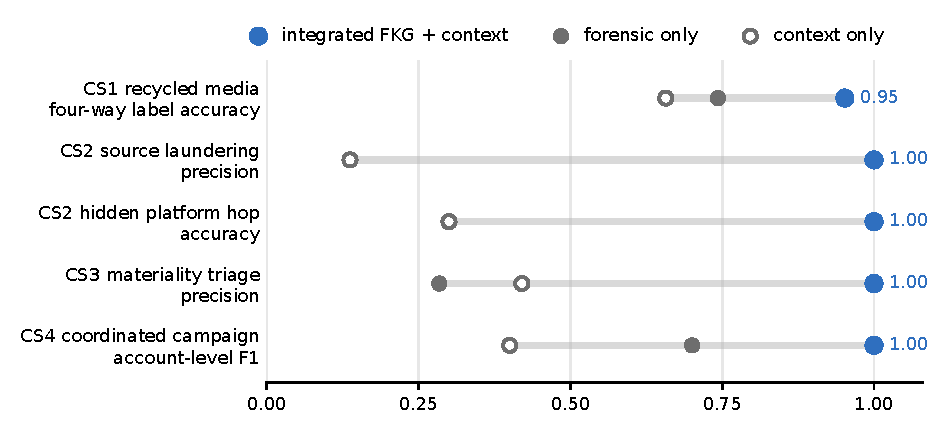
\includegraphics[width=\linewidth]{figures/headline.pdf}
\caption{Headline results, one row per investigative question. Every arm reads the same detector outputs.}
\end{figure}

\begin{itemize}
\item \textbf{The gain comes from integration, not detection.} Only the joins differ between arms. Forensics alone cannot see time, claims or accounts; context alone cannot see what was altered.
\item \textbf{Errors are misses, not false accusations.} Noise lowers recall while precision holds: 1.00 at every noise rate for CS3 triage, at least 0.81 for CS1 recycled-media flags up to $\eta = 0.5$. At $\eta = 0.5$, CS1 macro-F1 is 0.786 against 0.594 for forensics alone.
\item \textbf{Defence is a new query, not a new model.} In CS4, each attack that broke detection was answered by a new query over the same records: five of eleven fixed, two partly, four open.
\item \textbf{The schema is enough for agents.} On held-out worlds, agent-written queries score 0.92 to 0.96 against 0.91 for the hand-written set.
\end{itemize}

\section*{How it works}
\begin{figure}[htbp]\centering
% Architecture of the proposal: the FKG record joined to four context layers by shared identifiers.
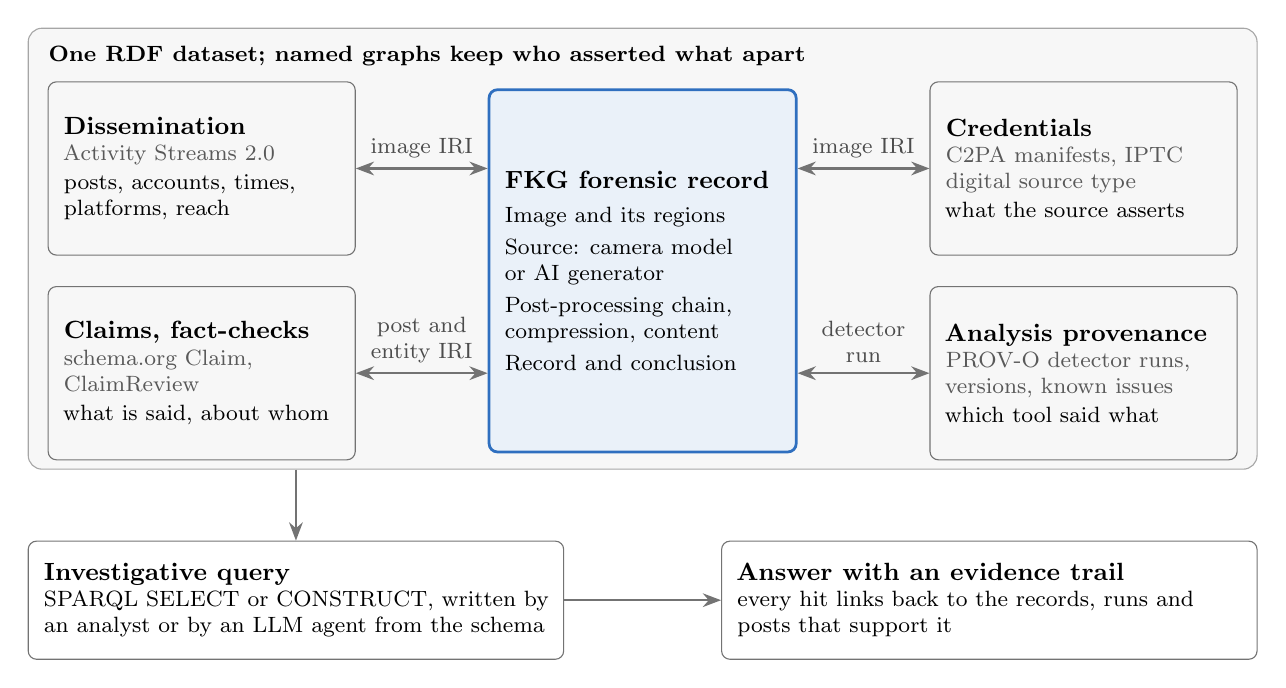
\begin{tikzpicture}[
  font=\footnotesize, >=Stealth,
  box/.style={draw=black!55, rounded corners=3pt, minimum width=3.9cm, align=flush left, inner sep=5pt, text width=3.5cm, font=\footnotesize},
  main/.style={box, draw=fkgblue, fill=fkgblue!10, line width=1pt},
  head/.style={font=\small\bfseries},
  std/.style={font=\footnotesize\color{black!65}},
  key/.style={font=\footnotesize\color{black!70}, align=center},
  link/.style={<->, draw=black!55, thick}]
  \node[main, minimum height=4.6cm] (fkg) at (0,0) {{\small\bfseries FKG forensic record}\\[3pt]
    Image and its regions\\[2pt] Source: camera model\\ or AI generator\\[2pt] Post-processing chain,\\ compression, content\\[2pt] Record and conclusion};
  \node[box, minimum height=2.2cm] (dis) at (-5.6, 1.3) {{\small\bfseries Dissemination}\\ {\footnotesize\color{black!65}Activity Streams 2.0}\\[1pt] posts, accounts, times, platforms, reach};
  \node[box, minimum height=2.2cm] (cla) at (-5.6,-1.3) {{\small\bfseries Claims, fact-checks}\\ {\footnotesize\color{black!65}schema.org Claim, ClaimReview}\\[1pt] what is said, about whom};
  \node[box, minimum height=2.2cm] (cre) at ( 5.6, 1.3) {{\small\bfseries Credentials}\\ {\footnotesize\color{black!65}C2PA manifests, IPTC digital source type}\\[1pt] what the source asserts};
  \node[box, minimum height=2.2cm] (pro) at ( 5.6,-1.3) {{\small\bfseries Analysis provenance}\\ {\footnotesize\color{black!65}PROV-O detector runs, versions, known issues}\\[1pt] which tool said what};
  \draw[link] (dis.east) -- node[key, above] {image IRI} (dis.east -| fkg.west);
  \draw[link] (cla.east) -- node[key, above] {post and\\entity IRI} (cla.east -| fkg.west);
  \draw[link] (cre.west) -- node[key, above] {image IRI} (cre.west -| fkg.east);
  \draw[link] (pro.west) -- node[key, above] {detector\\run} (pro.west -| fkg.east);
  \begin{scope}[on background layer]
    \node[draw=black!35, fill=black!3, rounded corners=5pt, inner sep=7pt, fit=(dis)(cla)(cre)(pro)(fkg), yshift=8pt, minimum height=5.6cm] (ds) {};
  \end{scope}
  \node[font=\footnotesize\bfseries, anchor=north west] at ([xshift=4pt,yshift=-3pt]ds.north west) {One RDF dataset; named graphs keep who asserted what apart};
  \node[box, text width=6.4cm, minimum width=6.8cm, minimum height=1.5cm, anchor=north west] (q) at ([yshift=-0.9cm]ds.south west) {{\small\bfseries Investigative query}\\ SPARQL SELECT or CONSTRUCT, written by an analyst or by an LLM agent from the schema};
  \node[box, text width=6.4cm, minimum width=6.8cm, minimum height=1.5cm, anchor=north east] (a) at ([yshift=-0.9cm]ds.south east) {{\small\bfseries Answer with an evidence trail}\\ every hit links back to the records, runs and posts that support it};
  \draw[->, draw=black!55, thick] (q.north |- ds.south) -- (q.north);
  \draw[->, draw=black!55, thick] (q.east) -- (a.west);
\end{tikzpicture}

\caption{Architecture. The FKG record is unchanged; everything around it reuses an existing standard. Labels on the arrows are the join keys.}
\end{figure}

\begin{itemize}
\item \textbf{Three identifiers do the joining:} the image IRI (post, credential, FKG record), the entity IRI (claim subject and altered content) and the detector run (FKG record and the fact-check that cites it).
\item \textbf{Almost nothing is new vocabulary.} The forensic layer is FKG as published; the context layer borrows existing standards plus a handful of terms such as a platform's transcoding profile.
\item \textbf{Plain SPARQL 1.1, no reasoner.} SHACL validates every record.
\end{itemize}

\section*{Four case studies at a glance}
\begingroup\small\par\smallskip\noindent
\begin{tabularx}{\linewidth}{@{}>{\raggedright\arraybackslash}p{2.2cm}>{\raggedright\arraybackslash}X>{\raggedright\arraybackslash}X>{\raggedright\arraybackslash}p{2.3cm}>{\raggedright\arraybackslash}p{2.0cm}@{}}
\toprule
\textbf{Study} & \textbf{Investigative question} & \textbf{What the join adds} & \textbf{Integrated} & \textbf{Best single layer} \\
\midrule
CS1 Recycled media & Is an authentic photo presented as showing an event it predates? & Earliest near-duplicate copy against the claimed event date, guarded by camera-model agreement & 0.952 accuracy & 0.743 (forensic) \\
CS2 Lineage and laundering & Which copy added the AI region, which platform did a file pass through, who credits an outlet for an edit it never published? & Copies ordered by compression, resampling and inserted regions, then tied to posts and credits & Hop 50/50, laundering precision 1.00 & 15/50, 0.137 (context) \\
CS3 Materiality and intent & Does an undisclosed alteration touch what the claim is about? & Altered content's entity against the claim's subject and the credential & Precision 1.00 at recall 0.912 & 0.420 (context) \\
CS4 Coordinated campaign & Which accounts run a coordinated campaign with manipulated media? & Shared generator and processing recipe (a forensic TTP) plus narrative and timing & F1 1.00 (0.97 at $\eta = 0.7$) & 0.70 (forensic) \\
\bottomrule
\end{tabularx}
\par\medskip\endgroup

The graph also audits its own analysis (CS3). It finds all 8 credentials the forensics contradict, all 3 attributions to a generator not yet released, and all 5 fact-checks that rest on a faulty detector version.

\section*{Decisions the paper needs from Jane}
CS1 to CS3 and CS4 were built in parallel and made different, reversible encoding choices. The six that matter most:

\begingroup\small\par\smallskip\noindent
\begin{tabularx}{\linewidth}{@{}>{\raggedright\arraybackslash}p{4.0cm}>{\raggedright\arraybackslash}X>{\raggedright\arraybackslash}p{2.9cm}@{}}
\toprule
\textbf{Decision} & \textbf{Question} & \textbf{Our suggestion} \\
\midrule
Where new terms live & Should the context vocabulary join FKG 0.2, or ship as a profile that imports it? & Open \\
Fully synthetic images & A verdict value, a manipulation type, or both? & One shared term \\
Named graphs & Per forensic record, per producer, or both? & Per producer \\
Statement-level provenance & Named graphs, or RDF 1.2 triple terms? & Open \\
Image identifiers & Adopt content-derived \code{ni:///sha-256} IRIs? & Adopt \\
Entities on content & Should Content carry entity IRIs natively? CS3 depends on it. & Adopt \\
\bottomrule
\end{tabularx}
\par\medskip\endgroup

Four smaller ones (compression subclasses, axioms SHACL cannot check, a shared reliability threshold, where an intent assessment belongs) are in §8 of the full report.

\section*{Caveats}
\begin{itemize}
\item \textbf{Synthetic only.} The numbers show that queries recover planted structure, not how an FKG pipeline performs on real media. The paper's evaluation should open with this.
\item \textbf{Circularity risk.} One author built the worlds and the hand-written queries. Agents that never saw those queries, fresh seeds and held-out worlds mitigate it.
\item \textbf{Leaks found and fixed.} Both simulators first leaked ground truth into readable attributes. After the fix, no single attribute predicts truth above about 0.67 balanced accuracy.
\item \textbf{Upper bounds by design.} A pasted region's single-compression trace is recorded without noise, and CS4's processing-chain detection rates are assumed.
\item \textbf{Hardest question.} CS2 patient zero reaches precision 0.75 (F1 0.56 across ten seeds): a detector false positive that recurs on copies looks like corroboration.
\item \textbf{Scale.} Worlds hold 10k to 745k quads; real crawls need incremental candidates and materialised rules.
\end{itemize}

\section*{Next experiments and code}
\begingroup\small\par\smallskip\noindent
\begin{tabularx}{\linewidth}{@{}>{\raggedright\arraybackslash}X>{\raggedright\arraybackslash}X>{\raggedright\arraybackslash}p{1.3cm}@{}}
\toprule
\textbf{Experiment} & \textbf{What it would establish} & \textbf{Effort} \\
\midrule
Real FKG pipeline on public out-of-context and provenance benchmarks & The joins still help with real detector outputs & Medium \\
Join real published fact-checks to the images they cite & The claim layer works on messy real claims & Medium \\
Settle the decisions; release FKG 0.2, the profile, shapes and 18 competency questions & A reusable benchmark for query-based investigation & Low \\
Controlled agent study: several models, repeated runs, notes with and without caveats & How reliably agents produce correct, affordable queries & Medium \\
\bottomrule
\end{tabularx}
\par\medskip\endgroup

\textbf{Code:} private GitHub repository \href{https://github.com/ductai199x/fkg-case-studies}{ductai199x/fkg-case-studies}, managed with uv. After \code{uv sync}, \code{make all} rebuilds every world and result, and \code{make check} audits every SPARQL query and reruns the quoted numbers; \code{make sweep} and \code{make agents} run separately. §11 of the full report lists one command per result.
\end{document}
